\documentclass[oneside, 11pt]{article}

\usepackage[T1]{fontenc}
\usepackage[utf8]{inputenc}
\usepackage[english]{babel}

\usepackage{fouriernc}
\usepackage[detect-all, binary-units, separate-uncertainty=true,
            per-mode=symbol, retain-explicit-plus, retain-unity-mantissa=false]{siunitx}

\usepackage{setspace}
\setstretch{1.2}

\setlength{\parskip}{\smallskipamount}
\setlength{\parindent}{0pt}

\usepackage[headheight=14pt]{geometry}
\geometry{marginparwidth=0.5cm, verbose, a4paper, tmargin=3cm, bmargin=3cm,
          lmargin=2cm, rmargin=2cm}

\usepackage{float}

\usepackage[fleqn]{amsmath}
\numberwithin{equation}{section}
\numberwithin{figure}{section}

\usepackage{graphicx}
\graphicspath{{images/}{../../../images/}}

\usepackage{tikz}
\usetikzlibrary{shapes}
\usetikzlibrary{plotmarks}

\newcounter{Exercise}
\setcounter{Exercise}{1}
\usepackage{xcolor}
\definecolor{shadecolor}{gray}{0.9}
\usepackage{framed}
\usepackage{caption}

\usepackage{url}


\usepackage{fancyhdr}
\pagestyle{fancy}
\fancyhf{}
\rhead{\thepage}
\renewcommand{\footrulewidth}{0pt}
\renewcommand{\headrulewidth}{0pt}

\fancypagestyle{firststyle}
{
    \fancyhf{}
    \rhead{\thepage}
    \cfoot{
\includegraphics[height=30pt]{HiSPARClogo}}
    \rfoot{
\includegraphics[height=25pt]{CCbysa}}
    \lfoot{
\includegraphics[height=30pt]{NIKHEFlogo}}
    \renewcommand{\footskip}{50pt}
    \renewcommand{\footrulewidth}{0.1pt}
    \renewcommand{\headrulewidth}{0pt}
}

\newcommand{\figref}[1]{Figuur~\ref{#1}}

\newcommand{\hisparc}{\textsmaller{HiSPARC}\xspace}
\newcommand{\kascade}{\textsmaller{KASCADE}\xspace}
\newcommand{\sapphire}{\textsmaller{SAPPHiRE}\xspace}
\newcommand{\jsparc}{\textsmaller{jSparc}\xspace}
\newcommand{\hdf}{\textsmaller{HDF5}\xspace}
\newcommand{\aires}{\textsmaller{AIRES}\xspace}
\newcommand{\csv}{\textsmaller{CSV}\xspace}
\newcommand{\python}{\textsmaller{PYTHON}\xspace}
\newcommand{\corsika}{\textsmaller{CORSIKA}\xspace}
\newcommand{\labview}{\textsmaller{LabVIEW}\xspace}
\newcommand{\daq}{\textsmaller{DAQ}\xspace}
\newcommand{\adc}{\textsmaller{ADC}\xspace}
\newcommand{\hi}{\textsc{h i}\xspace}
\newcommand{\hii}{\textsc{h ii}\xspace}
\newcommand{\mip}{\textsmaller{MIP}\xspace}
\newcommand{\hisparcii}{\textsmaller{HiSPARC II}\xspace}
\newcommand{\hisparciii}{\textsmaller{HiSPARC III}\xspace}

\DeclareSIUnit{\electronvolt}{\ensuremath{\mathrm{e\!\!\:V}}}

\DeclareSIUnit{\unitsigma}{\ensuremath{\sigma}}
\DeclareSIUnit{\mip}{\textsmaller{MIP}}
\DeclareSIUnit{\adc}{\textsmaller{ADC}}

\DeclareSIUnit{\gauss}{G}
\DeclareSIUnit{\parsec}{pc}
\DeclareSIUnit{\year}{yr}




%document details
\author{N.G. Schultheiss \\ translated and adapted by K. Schadenberg}
\date{}
\title{Compton}


\begin{document}
\maketitle

\section{Introduction}
How do photons and electrons behave during collisions? That is the subject of this module. Photons always move with the speed of light, but electrons can also have a very high speed after collisions. It is therefore advised to first read through the modules `Collisions' and `Relativity' before starting with this text.

\section{Compton}
Arthur Holly Compton was researching the scattering behaviour of X-rays. He discovered that this scattering has to do with photons colliding with electrons. This type of scattering is now called Compton scattering. In later research he focussed on the distribution of (intensity of) cosmic radiation on Earth.

In Compton scattering a small part of the energy and momentum of a photon is transferred to an electron. The law of conservation of energy and the law of conservation of momentum both play an important part during this `collision'. If a photon collides with a free electron (i.e. not bound to a nucleus) all energy can be used to accelerate the electron. In this case the collision is elastic. If the electron were bound to a nucleus, then first this bond must be broken to create an ion. In this case the collision is no longer elastic.

Lets take a look at a stationary, unbound electron:
\begin{align}
E_{\mbox{electron}} &= m_{\mbox{electron}}c^2 \\
p_{\mbox{electron}} &= 0 \label{eq:E_e}
\end{align}
The photon headed for the electron:
\begin{align}
E_{\mbox{photon}} &= h \nu\\
p_{\mbox{photon}} &= \frac{h \nu}{c} \label{eq:E_ph}
\end{align}
After the collision the electron has a certain momentum and energy, this means the photon lost some of its energy and momentum. This situation is drawn in figure~\ref{fig:coll}

\begin{figure}\begin{center}
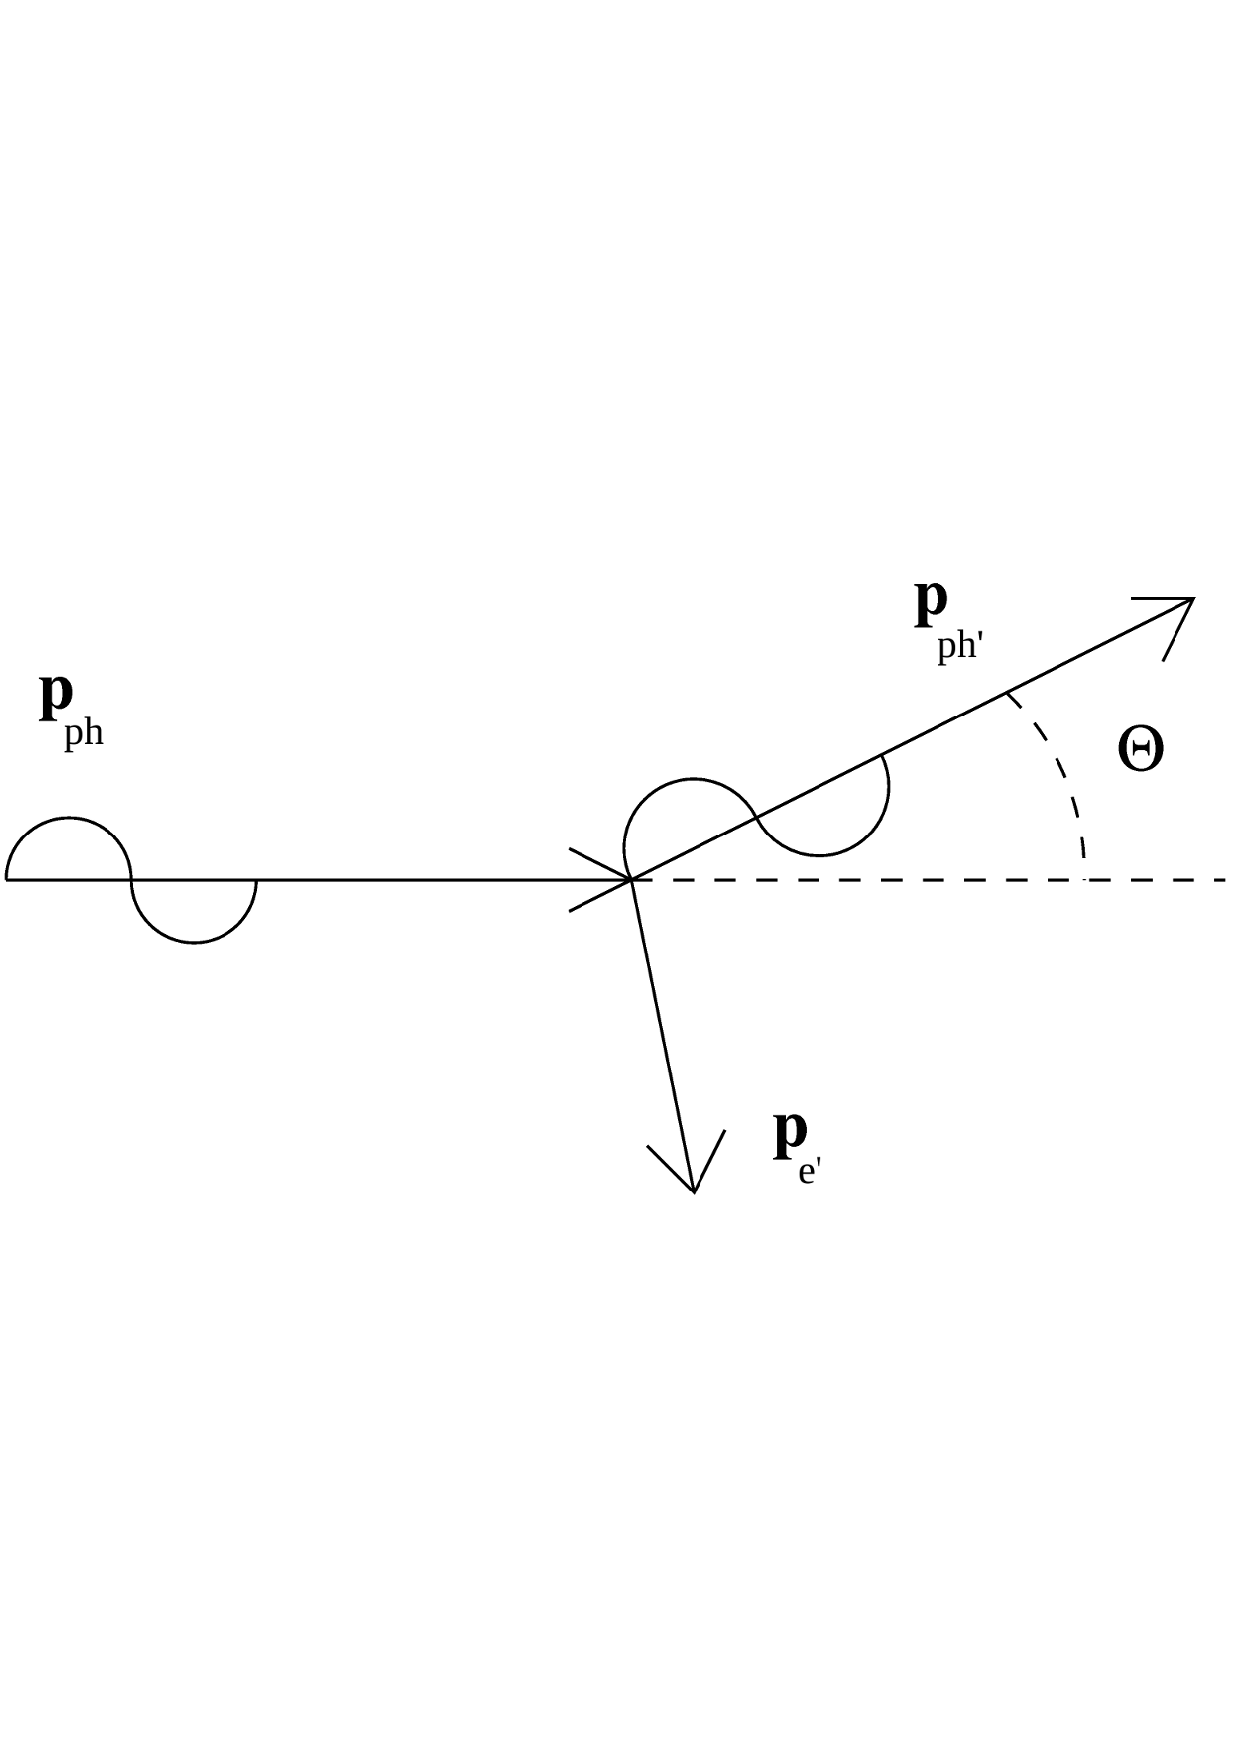
\includegraphics[scale=3]{compton}%
\caption{Compton scattering.}\label{fig:coll}
\end{center}\end{figure}

The law of conservation of momentum allows us to write:
\begin{equation}
\textbf{p}_{ph} = \textbf{p}_{ph'} + \textbf{p}_{e'}
\end{equation}
Rearranging the vectors a bit allows us to use the cosine rule:
\begin{equation}
p^2_{e'} = p^2_{ph} + p^2_{f'} - 2p_{ph}p_{ph'}\cos(\theta) \label{eq:en_final}
\end{equation}
The law of conservation of energy allows us to write:
\begin{equation}
E_{ph} +E_e = E_{ph'} + E_{e'}
\end{equation}
We rewrite this equation using the notation for energy from equations~\ref{eq:E_e} and \ref{eq:E_ph}:
\begin{align}
h \nu_{ph} + m_e c^2 &= h \nu_{ph'} + \sqrt{p^2_{e'}c^2 + m^2_e c^4} \Longleftrightarrow\\
h \nu_{ph} - h \nu_{ph'} + m_e c^2 &= \sqrt{p^2_{e'}c^2 + m^2_e c^4}
\end{align}
Squaring both sides yields:
\begin{align}
\left( h \nu_{ph} - h \nu_{ph'} + m_e c^2 \right)^2 &= p^2_{e'}c^2 + m^2_e c^4 \Longleftrightarrow\\
\left( h \nu_{ph} - h \nu_{ph'} \right)^2 + 2m_e c^2 \left( h \nu_{ph} - h \nu_{ph'}\right) + m^2_e c^4 &= p^2_{e'}c^2 + m^2_e c^4 \Longleftrightarrow\\
h^2\nu^2_{ph} - 2h^2\nu_{ph}\nu_{ph'} + h^2\nu^2_{ph'} + 2m_ec^2 \left( h\nu_{ph} - h\nu_{ph'} \right) &= p^2_{e'}c^2 \Longleftrightarrow\\
\frac{h^2\nu^2_{ph}}{c^2} - \frac{2h^2\nu_{ph}\nu_{ph'}}{c^2} + \frac{h^2\nu^2_{ph'}}{c^2}+ 2m_ec^2 \left(  \frac{h\nu_{ph}}{c^2} - \frac{h\nu_{ph'}}{c^2} \right) &= p^2_{e'} \label{eq:mom_final}
\end{align}

Combining the law of conservation energy (\ref{eq:en_final}) with the law of conservation of momentum (\ref{eq:mom_final}):
\begin{align}
\begin{aligned} \nonumber
\frac{h^2\nu^2_{ph}}{c^2} - \frac{2h^2\nu_{ph}\nu_{ph'}}{c^2} + \frac{h^2\nu^2_{ph'}}{c^2} & \\
+ 2m_ec^2 \left( \frac{h\nu_{ph}}{c^2} - \frac{h\nu_{ph'}}{c^2} \right) & = p^2_{ph} + p^2_{ph'} - 2p_{ph}p_{ph'}\cos(\theta) \Longleftrightarrow \\
\end{aligned} \\ 
\begin{aligned}
- \frac{2h^2\nu_{ph}\nu_{ph'}}{c^2} + 2m_ec^2 \left( \frac{h\nu_{ph}}{c} - \frac{h\nu_{ph'}}{c} \right) &= \frac{2h^2 \nu_{ph}\nu_{ph'}}{c^2} \cos(\theta) \Longleftrightarrow\\
2m_ec^2 \left( \frac{h\nu_{ph}}{c} - \frac{h\nu_{ph'}}{c} \right) &= \frac{2h^2 \nu_{ph}\nu_{ph'}}{c^2} \left( 1-\cos(\theta) \right) \Longleftrightarrow\\
\frac{m_ec}{h} \left( \frac{\nu_{ph}}{c} - \frac{\nu_{ph'}}{c} \right) &= \frac{\nu_{ph}\nu_{ph'}}{c^2} \left( 1-\cos(\theta) \right) \Longleftrightarrow\\
\frac{m_ec}{h} \left( \frac{c}{\nu_{ph'}} - \frac{c}{\nu_{ph}} \right) &= \left(  1-\cos(\theta) \right) \Longleftrightarrow\\
\left( \frac{c}{\nu_{ph'}} - \frac{c}{\nu_{ph}} \right) &= \frac{h}{m_ec} \left(  1-\cos(\theta) \right) \Longleftrightarrow\\
\Delta \lambda &= \frac{h}{m_ec} \left( 1-\cos(\theta) \right)
\end{aligned}
\end{align}
This final equation gives the scattering of photons by electrons. De constant $\frac{h}{m_ec}$ is known as the Compton wavelength of the electron.

After the collision between the photon and the electron, the electron is no longer stationary. This can lead to all kinds of effects. Free electrons moving in a saturated vapour can lead to condensation along the path of the electrons. This is exactly what Charles Thomson Rees Wilson saw when he was experimenting with the formation of clouds. This effect is used in a cloud chamber to view (the effects of) cosmic radiation. You can read more about this in the module `van der Waals \& Wilson'.

\end{document}
